\section{Embedded Systems}

%----------------------------------------------------------------------------------------
%	DEFINITION SUBSECTION
%----------------------------------------------------------------------------------------

\subsection{Definition}
An Embedded system is a combination of computer hardware and software. As with any electronic system, this system requires a hardware platform and that is built with a microprocessor or micro-controller.The Embedded system hardware includes elements like user interface, Input/Output interfaces, display and memory, etc.Generally, an embedded system comprises power supply, processor, memory, timers, serial  communication ports and system application specific circuits.

%----------------------------------------------------------------------------------------
%	DEFINITION SUBSECTION
%----------------------------------------------------------------------------------------

\subsection{Types}
Embedded systems can be classified into different types based on performance, functional requirements and performance of the micro-controller.\\

\centerline{
	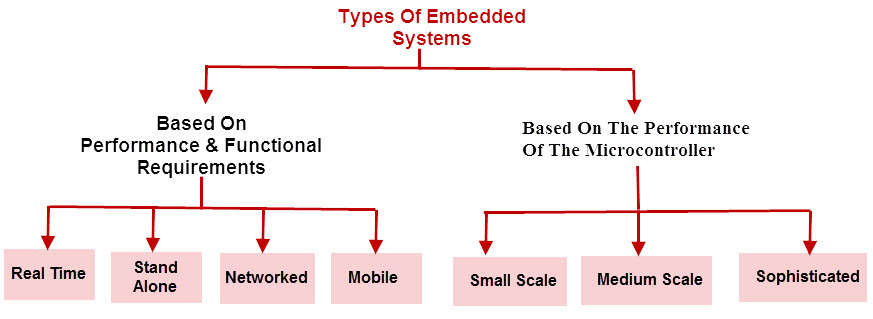
\includegraphics[width=1.0\textwidth]{overview/images/types.jpg}
}

\begin{enumerate}

\item Embedded systems are classified into four categories based on their performance and functional requirements:

\begin{itemize}
  \item Stand alone embedded systems
  \item Real time embedded systems
  \item Networked embedded systems
  \item Mobile embedded systems
\end{itemize}

\newpage
\item Embedded Systems are classified into three types based on the performance of the micro-controller such as

\begin{itemize}
  \item Small scale embedded systems
  \item Medium scale embedded systems
  \item Sophisticated embedded systems
\end{itemize}

\end{enumerate}

